\subsection{Dimensionamento mediante criterio termico di una conduttura elettrica}
Una conduttura elettrica può essere dimensionata mediante differenti criteri, come 
quello termico, quello del massimo rendiconto economico o quello che minimizza l'ingombro 
o le perdite.

Si stabilisce la massima corrente stazionaria che un conduttore può sostenere
senza che subisca danneggiamenti per sé stesso o i corpi circostanti.

Si assume che il conduttore sia una struttura filiforme, prodotta da una sezione
piana che si muove lungo una linea passante per il suo baricentro, un cilindro a sezione
variabile con asse la suddetta linea $\Gamma$.

Il conduttore può essere rivestito con un materiale isolante o immerso in un fluido come
olio minerale o aria.

La lunghezza del conduttore non ha influenza sulla portata mentre la sezione 
può essere adattata allo specifico carico meccanico a cui il conduttore sarà sottoposto,
tipicamente i conduttori richiedono flessibilità e le sezioni sono di tipo filiforme
intrecciati, in una stazione di trasformazione invece, date le elevate potenze in gioco
possono essere utilizzati dei conduttori a sbarra ai quali possono essere agganciate
le varie diramazioni.

Il grado di libertà elettrico rimasto è l'area della sezione, area che verrà dimensionata
nella prossima analisi.

Ogni volta che una corrente attraversa un conduttore, questo si riscalda per effetto Joule
$$
P_R^{(a)} = Ri^2 = \iiint_C \eta |\vec{J}|^2 dV \geq 0
$$
Questa dissipazione converte il lavoro compiuto dal campo elettromagnetico per
spostare i portatori di carica in calore fornito al corpo, al reticolo metallico.

Per conduttori rivestiti il riscaldamento per effetto Joule può danneggiare gli isolanti
per questo motivo esiste una temperatura limite dell'isolante.
Si riportano le seguenti temperature di riferimento:
\begin{itemize}
\item cotone-carta non immersi in olio
pari a circa \SI{90}{\celsius} a cui vanno sottratti 10 o 20 \si{\celsius} se questa
viene misurata dall'esterno.
\item cotone-carta immersi in olio $T_{max} \simeq \SI{105}{\celsius}$
\item conduttori in aria $T_{max} \simeq 70\div 80\ \si{\celsius}$
\item conduttori da riscaldamento (stufe o forni) $T_{max} \simeq 400,600,1100\ \si{\celsius} $ a seconda della lega (Cu-Ni, Fe-Ni, Cr-Ni) 
\end{itemize}

Anche i conduttori nudi presentano lo stesso problema anche se in maniera ridotta, sono però 
presenti delle giunzioni lungo la linea che uniscono i conduttori in parallelo, per questo
motivo non si può in ogni caso superare la temperatura di 
\SI{180}{\celsius}

\paragraph{Andamento del riscaldamento di un conduttore}
Per analizzare con semplicità l'andamento della temperatura di un conduttore attraversato
da corrente è necessario eseguire una serie di ipotesi semplificative che non intaccano
gli ordini di grandezza dei risultati.

\begin{itemize}
\item Si considera una temperatura media del conduttore, ossia conduttore uniforme,
altrimenti se ne dovrebbe studiare il campo di temperatura
\item La capacità termica $Q$ $[\si{\joule\per\celsius}]$ indica la relazione tra il calore 
fornito al corpo e la sua variazione di temperatura, questa capacità termica è costante
\item Il fluido in cui`è immerso il conduttore è omogeneo e si trova ad una certa distanza
ad una temperatura ambiente $T_a$ fissata
\item Il calore emesso nell'unità di tempo dal corpo è proporzionale alla differenza 
$T-T_a$
\end{itemize}

La potenza termica assorbita dal conduttore è pari alla potenza elettrica assorbita
nell'intervallo di tempo elementare
$$
P^{(a)} dt = Q(T-T_a) + H(T-T_a) dt
$$
Il coefficiente $H$ detto coefficiente di adduzione o adduttanza termica ha le dimensioni
$[\si{\watt\per\celsius}]$
Derivando rispetto al tempo
$$
P^{(a)} = Q \frac{d}{dt} (T-T_a) + H(T-T_a)
$$
Se si assume che $P, Q, H$ siano costanti allora quella ottenuta è un'equazione
differenziale lineare del primo ordine a coefficienti costanti, si può integrare 
$$
\frac{P^{(a)}}{H} = \frac{Q}{H} \frac{d}{dt} (T-T_a) + (T-T_a)
$$
dove $\frac{Q}{H}$ ha le dimensioni di un tempo ed è proprio la costante di tempo termica
di riscaldamento/raffreddamento del corpo.
$$
T-T_a = Be^{-\frac{t}{\tau}} + \frac{P^{(a)}}{H}
$$
$B$ è una costante di integrazione determinabile con le condizioni iniziali es.
$T(t=0) = T_i$
$$
T_i - T_a = B + \frac{P^{(a)}}{H} \Rightarrow B = T_i - \left(T_a + \frac{P^{(a)}}{H}\right) 
= T_i - T_\infty
$$
in conclusione
$$
T(t) - \cancel{T_a} = (T_i - T_\infty)e^{-\frac{t}{\tau}} + T_\infty - \cancel{T_a}
$$
Scomponendo i termini ottenuti
$$
T = \left(T_1-T_a-\frac{P^{(a)}}{H}\right)e^{-\frac{t}{\tau}} + T_a + \frac{P^{(a)}}{H} 
$$
$$
T = T_i e^{-\frac{t}{\tau}} + T_a - T_a e^{-\frac{t}{\tau}} + \frac{P^{(a)}}{H} 
\left(1 - e^{-\frac{t}{\tau}}\right)
$$
$$
T = (T_i - T_a)e^{-\frac{t}{\tau}} + T_a + \frac{P^{(a)}}{H} \left(1-e^{-\frac{t}{\tau}}\right)
$$
I primi due termini rappresentano l'evoluzione libera del sistema mentre l'ultimo esplica
l'evoluzione forzata, perché dipende dalla potenza elettrica fornita.

Si suppone che la potenza fornita sia una funzione gradino, si vede l'andamento della
temperatura del conduttore
$$
P^{(a)}(t) = P \left[u(t) - u(t-\Delta t)\right]
$$
\begin{figure}[H]
\centering
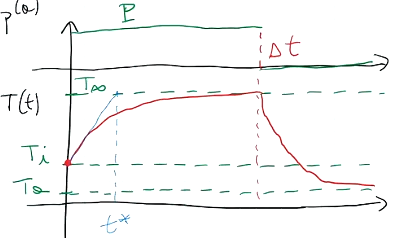
\includegraphics[width= 0.4\linewidth]{andamento_termico_conduttore}
\end{figure}
con $t^* = \tau$, si vede sviluppando la funzione in serie di Taylor al primo ordine
$$
T \simeq (T_i - T_a)\left(1-\frac{t}{\tau}\right) + T_a + \frac{P^{(a)}}{H}\left(-\frac{t}{\tau}\right)
$$
$$
T(t^*) = T_\infty \Rightarrow t^* = \tau
$$
$\tau$ rappresenta il tempo necessario al conduttore per raggiungere la temperatura 
di regime nell'ipotesi adiabatica. 
$$
P^{(a)} dt = Q(T-T_a)
$$
Invece per $t\geq 4\div 5 \tau$ resta la soluzione di regime
$$
P^{(a)}dt = H(T-T_a)dt \Rightarrow T_\infty - T_a = \frac{P^{(a)}}{H}
$$
L'incertezza principale di questa analisi riguarda la valutazione del coefficiente
$H$ di adduttanza termica, solitamente un problema che riguarda tutte e tre le tipologie
di scambio termico: conduzione, convezione e irraggiamento e che dipende linearmente
dalla superficie di scambio.

Il dimensionamento di un conduttore avviene dunque valutando la temperatura massima
di regime ammissibile, non è dunque rilevante il fenomeno transitorio.
$$
T_\infty - T_a = \frac{P^{(a)}}{H} = \frac{Ri^2}{H} \Rightarrow i_{\text{max}} = \sqrt{T_\infty-T_a\frac{kA}{R}}
$$
Sostituendo la legge di ohm per un conduttore filiforme
$$
i_{\text{max}} = \sqrt{T_\infty-T_a\frac{kA\cdot S}{\eta L}}
$$
e $T_{\text{max}}$ deve essere la massima temperatura ammissibile dall'isolante.
In generale 
$$
i_{\text{max}} = \sqrt{\left(T_\text{max} - T_a\right)\frac{k}{\eta}} \cdot \sqrt{\frac{A}{\text{Vol}}}\cdot S
$$
Ad esempio se si considera un cilindro rettilineo
\begin{align*}
A &= \pi d L \\
\text{Vol} &= \pi \frac{d^2}{4} L\\
\sqrt{\frac{A}{\text{Vol}}} &= \frac{2}{\sqrt{d}}
\end{align*}
Volendo calcolare la densità di corrente massima invece
$$
J_{\text{max}} = \frac{i_\text{max}}{S} = \sqrt{\left(T_\infty -T_a\right)\frac{kA\cancel{S}}{\eta S ^{\cancel{2}}L}} = \sqrt{\left(T_\infty -T_a\right)\frac{k}{\eta}\frac{A}{\text{Vol}}}
$$
In alternativa si può calcolare la sezione minima per condurre una certa corrente $i_\text{max}$
$$
S_\text{min} = \frac{i_\text{max}}{\sqrt{\left(T_\infty -T_a\right)\frac{k}{\eta}\frac{A}{\text{Vol}}}}
$$
Questa relazione è indipendente dalla forma della sezione.
Si nota inoltre che per grandi portate di corrente è più conveniente utilizzare cavi 
multipli piuttosto che un unico cavo di sezione maggiore.
Ad esempio un cavo cilindrico con $d = \sqrt{\frac{4S}{\pi}}$
$$
\sqrt{\frac{A}{\text{Vol}}} = \frac{2}{\sqrt{d}} = \frac{\sqrt[4]{16}}{\sqrt[4]{\frac{4S}{\pi}}} = \sqrt[4]{\frac{4\pi}{S}}
$$
Si considerino le seguenti dati
\begin{align*}
S &= 1,10,100,100\ \si{\milli\meter^2} \\
K &= \SI{10}{\watt\celsius^{-1}\meter^{-2}}\\
\left(T_\text{max}-T_a\right) &= \SI{30}{\celsius} \\
\gamma &= \SI{e7}{\siemens\per\meter} \Rightarrow \eta = \SI{e-7}{\ohm\meter}
\end{align*}
La densità di corrente massima sarà
$$
J_\text{max} = \sqrt{30\cdot\frac{10}{10^{-7}}}\cdot \sqrt[4]{\frac{4\pi}{S}} = \frac{10^5}{\sqrt[4]{S}} = 3.26,1.83,1.03,0.58 \ \si{\mega\ampere\per\meter^2}
$$
La portata invece
$$
i_\text{max} = J_\text{max}\cdot S = 3.26,18.3,103,580 \ \si{\ampere}
$$
Assegnata una $i_\text{max}$, il criterio termico suggerisce l'uso di $n$ conduttori
in parallelo, se $i_{\text{max}_2} = n\ i_{\text{max}_1}$ per avere la stessa portata
con un unico conduttore di sezione maggiore si avrebbe
$$
S_{\text{min}_2} = (n)^{\frac{4}{3}} S_{\text{min}_1}
$$
un aumento lineare della portata (numero di conduttori) comporta un aumento più che lineare 
della sezione equivalente necessaria
\begin{center}
\begin{tabular}{r c c c c}\centering
$n =$ & $2$ & $3$ & $6$ & $10$\\
$(n)^{\frac{4}{3}} =$ & $2.5$ & $4.3$ & $11$ & $21.5$
\end{tabular}
\end{center}
Il dimensionamento di una linea richiede quindi un giusto trade-off tra i costi dei
conduttori, il loro peso e il costo necessario all'installazione di conduttori multipli.
